\part{Validation and Results}

\chapter{Solution validation}

\section {Data model}

The model designed for the Observatory project represented in figure~\ref{fig:datamodel-obsproject} is a simplification of the ALMA Project Data Model summarized in section~\ref{sec:apdm} and it is the model used in the ALMA's Dynamic Scheduling Algorithm briefly described in section~\ref{sec:alma-dsa}.

The most relevant parts are: 
\begin{description}
\item[bla1] \hfill \\
Description of bla1
\end{description}

\begin{figure}[]	
\begin{center}
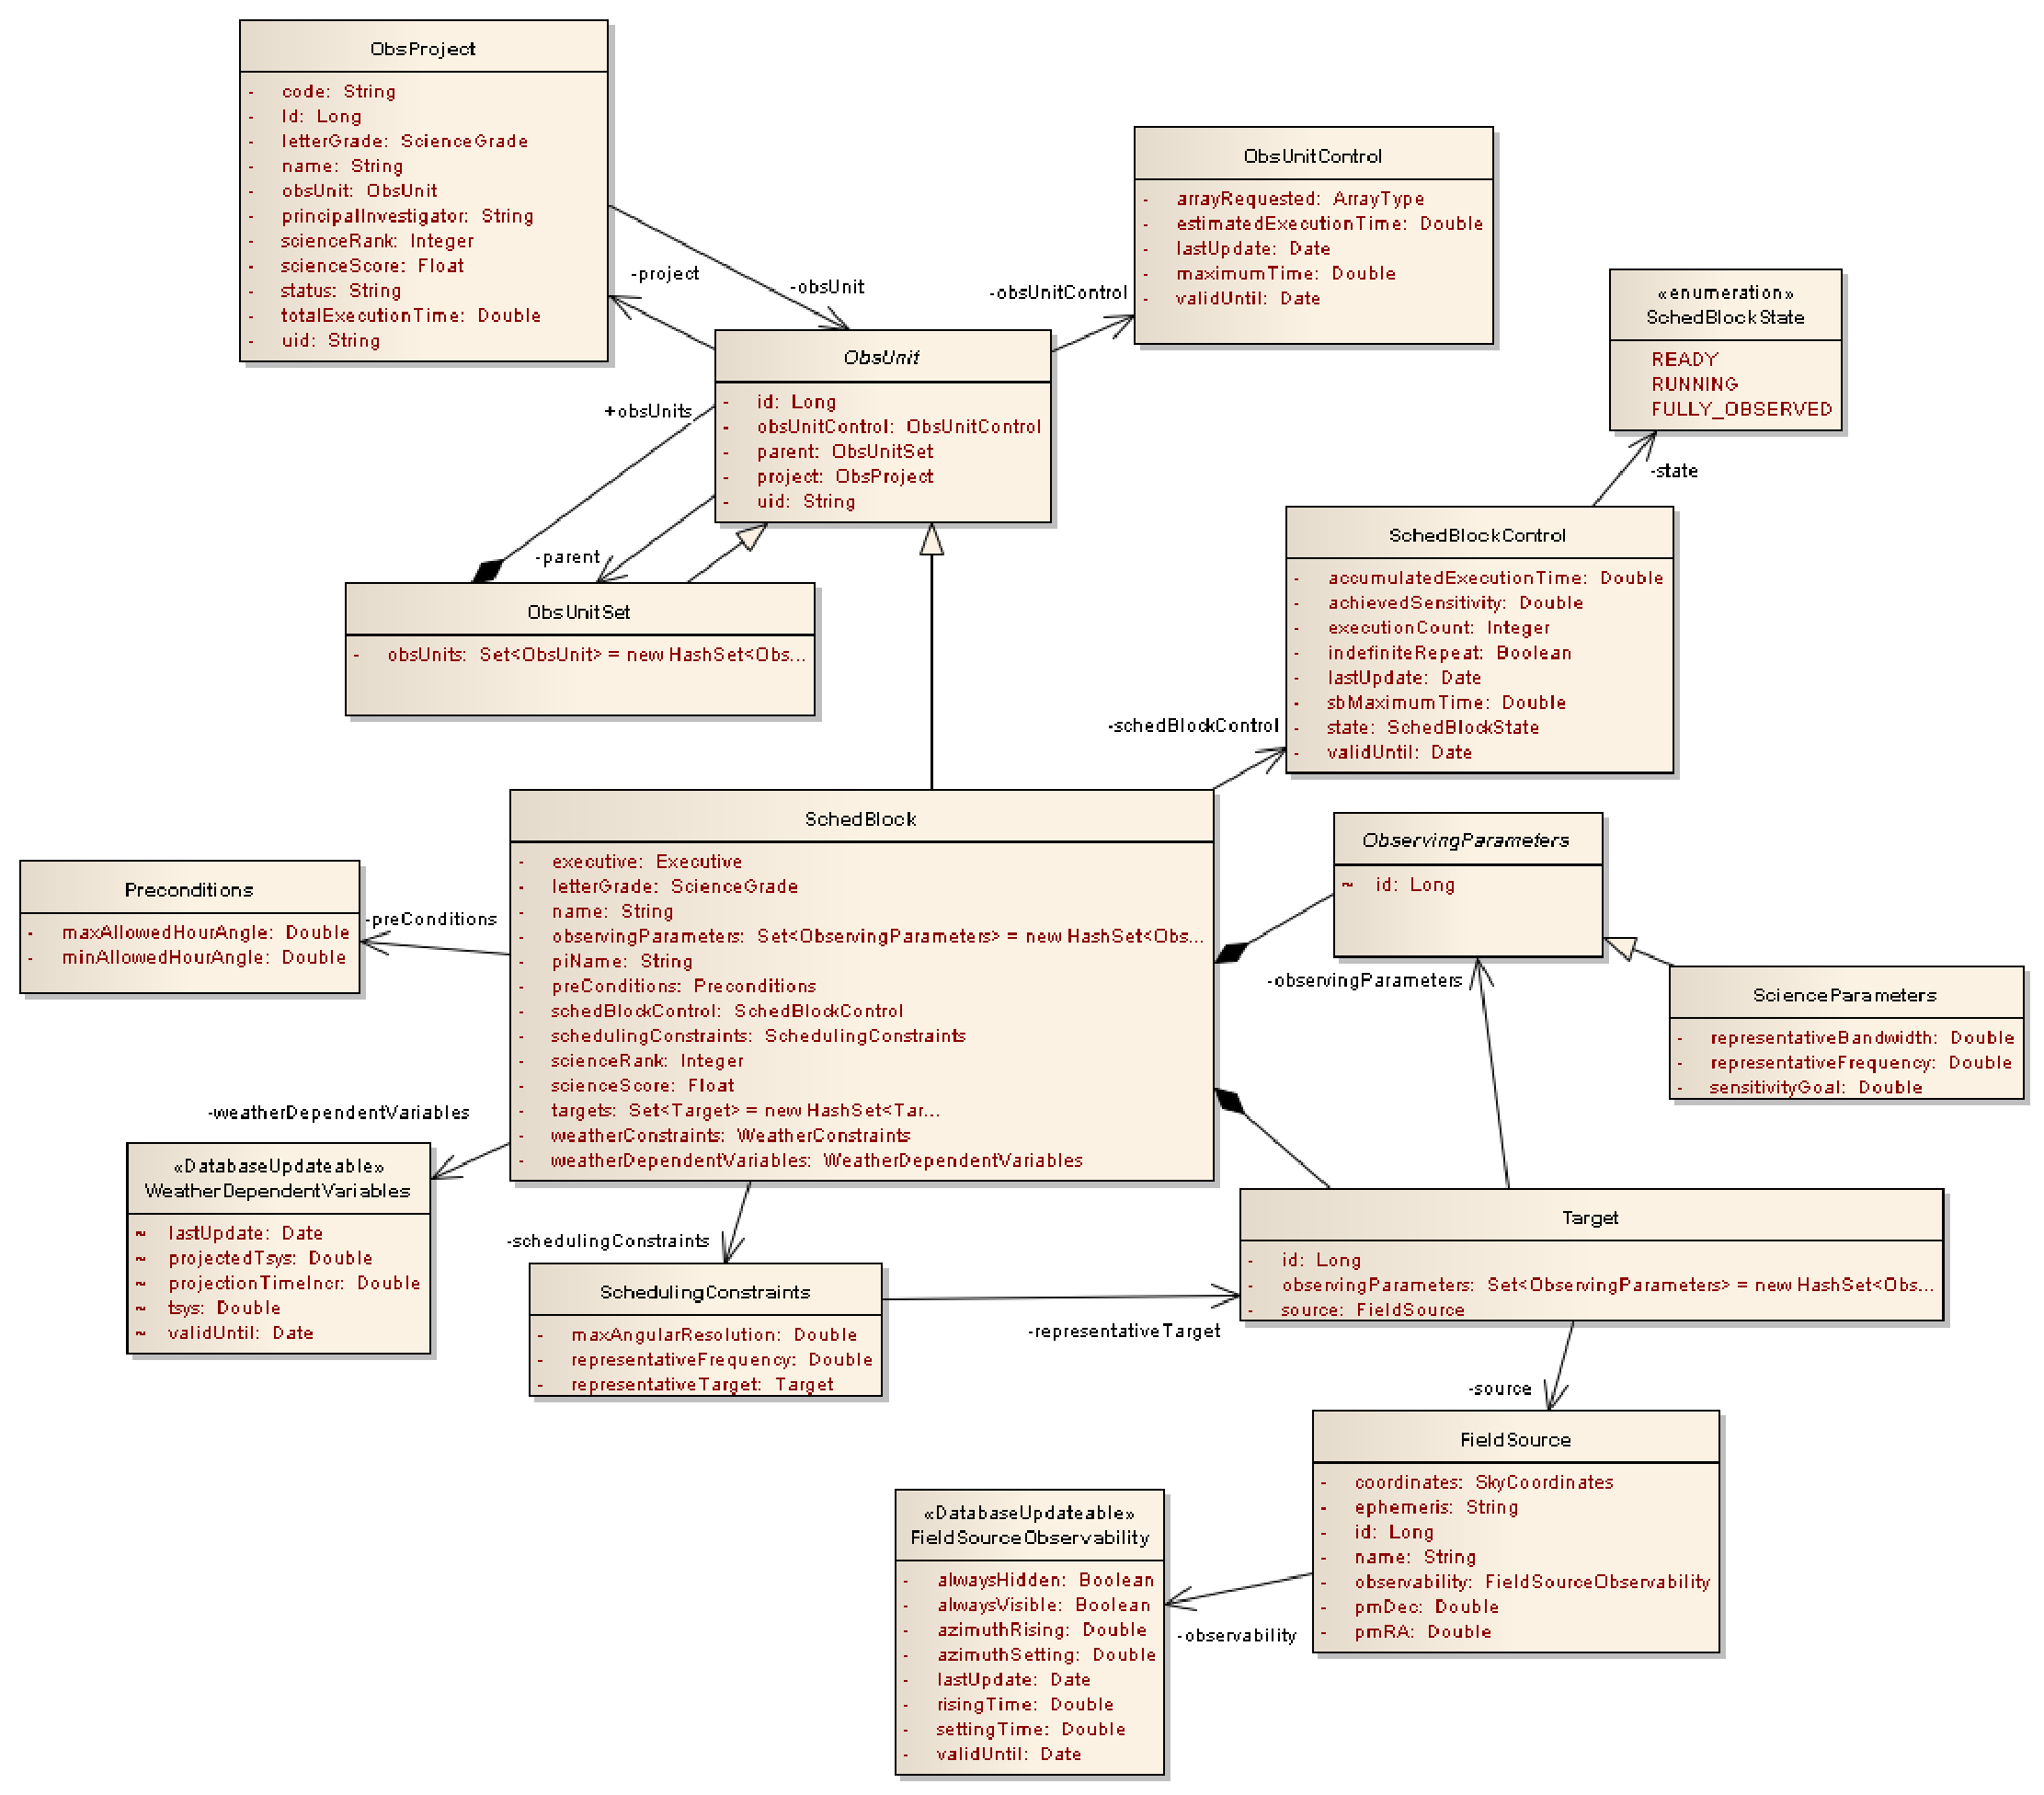
\includegraphics[width=1.15\textwidth]{images/ObsProject}
\caption{Observation Project data model}
\end{center}
\label{fig:datamodel-obsproject}
\end{figure}

The model designed for handle the observatory instrumentation is represented in figure~\ref{fig:datamodel-observatory}

\begin{figure}[]	
\begin{center}
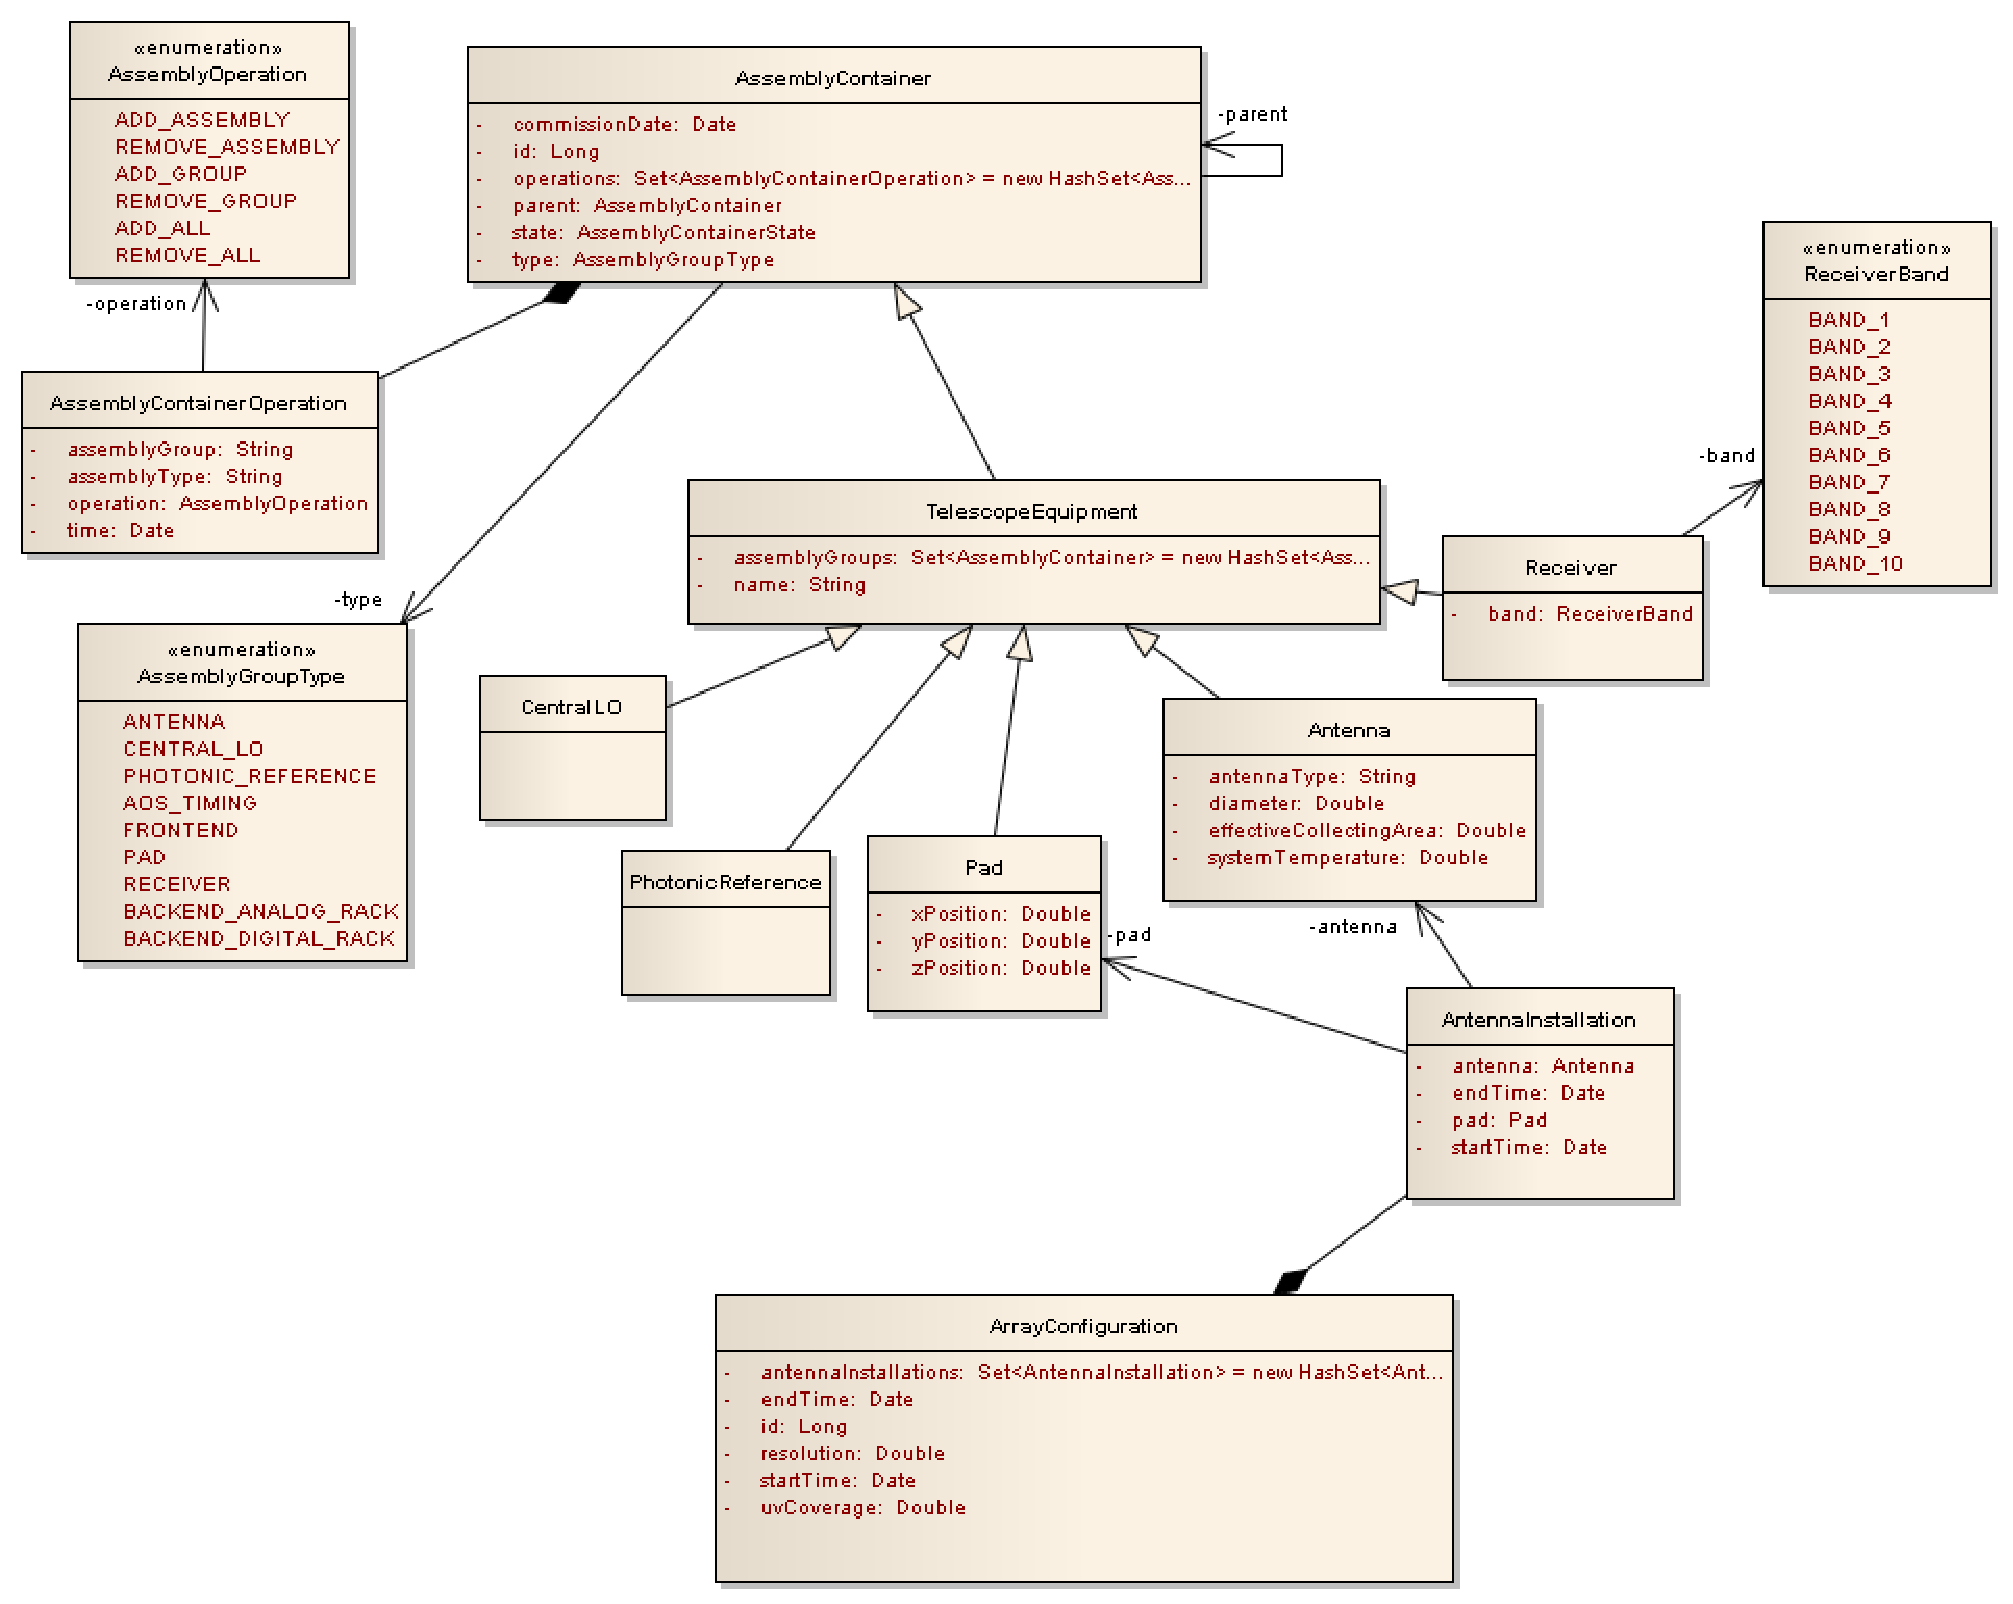
\includegraphics[width=\textwidth]{images/Observatory}
\caption{Observatory instrumentation data model}
\end{center}
\label{fig:datamodel-observatory}
\end{figure}

The model designed for handle the Executive information and the observing season is represented in figure~\ref{fig:datamodel-executive}

\begin{figure}[]	
\begin{center}
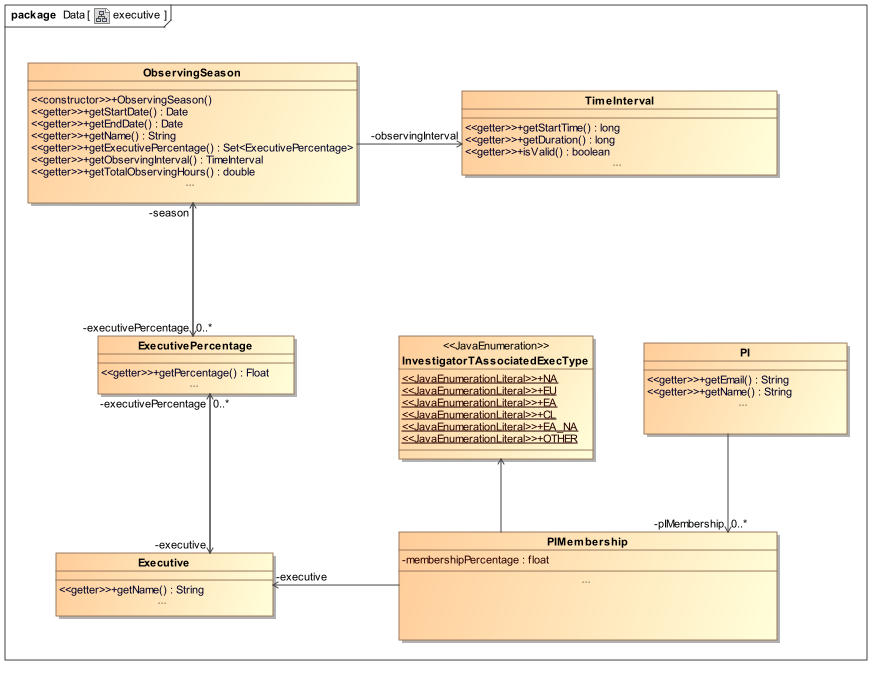
\includegraphics[width=\textwidth]{images/Executive}
\caption{Executive and observing season data model}
\end{center}
\label{fig:datamodel-executive}
\end{figure}

The model designed for handle the weather is represented in figure~\ref{fig:datamodel-weather}

\begin{figure}[]	
\begin{center}
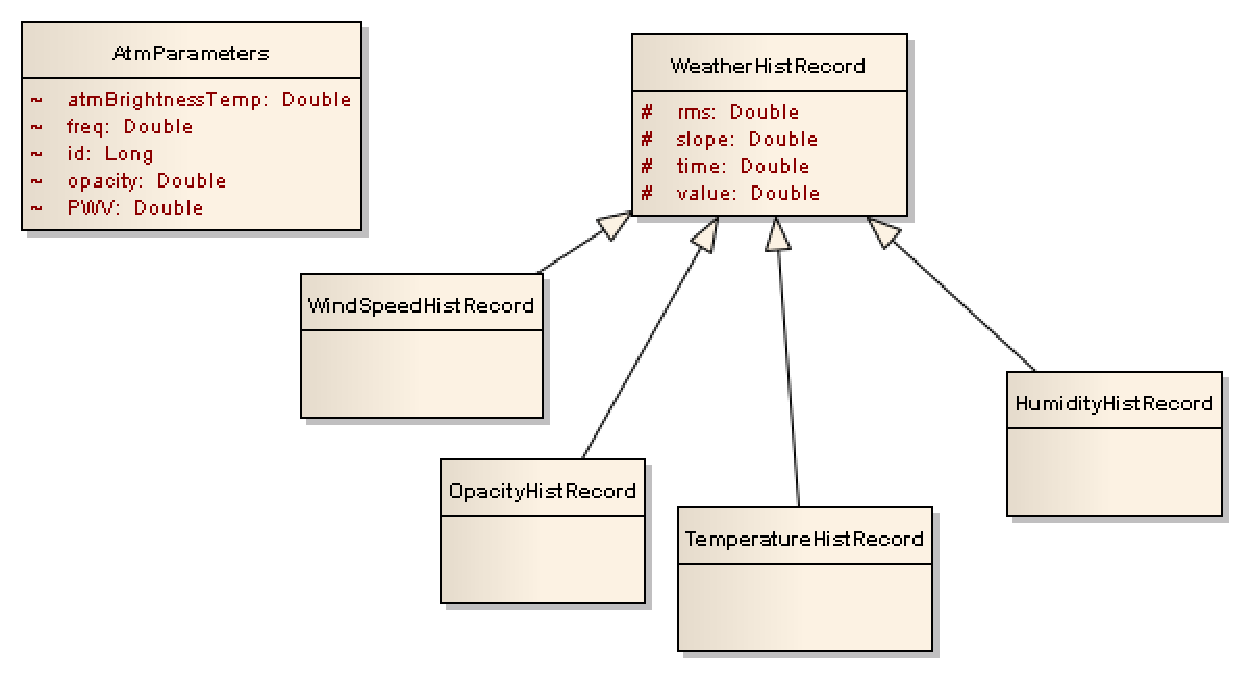
\includegraphics[width=0.6\textwidth]{images/Weather}
\caption{Executive and observing season data model}
\end{center}
\label{fig:datamodel-weather}
\end{figure}

\section {Simulation}
The simulator is the one used in the ALMA's scheduling subsystem. At the time when this document was written it remains mostly unchanged from its original design explained in detail in~\cite{hoffstadt10}. Nevertheless some modifications where done during the development of this work to support the simulation of several scenarios for the solution provided for the``Array configuration planning problem''. Next a briefly description of the simulator work-flow, shown in figure~\ref{fig:sim-state-machine}, is presented:

\begin{figure}[]	
\begin{center}
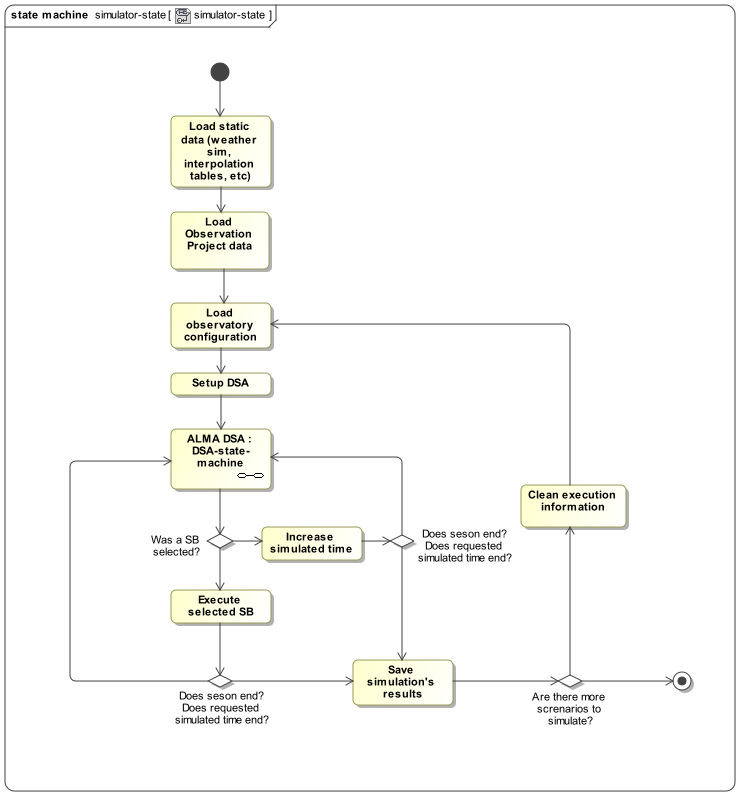
\includegraphics[width=0.8\textwidth]{images/simulator-state-machine}
\end{center}
\caption{ALMA simulator's state machine}
\label{fig:sim-state-machine}
\end{figure}

\begin{description}
\item[Load static data] \hfill \\
In this step the simulator will load all the immutable data from data-sources. This includes weather simulation data (temperature, humidity, wind speed, etc) and atmospheric interpolation tables to calculate the atmospheric opacity given the PWV and frequency. This step is separate from the rest of the date given that, the original ALMA's simulator is intended to be run using a relational database as back-end, then these data will load just once.

During the development of this work, the simulator has been modified to work with data loaded completely in memory. Therefore this step add no value to the simulator itself. However it is worth of mention the difference with the original simulator used in ALMA software. 

\item[Load Observation project data] \hfill \\
In this step the simulator will load the data intended to be modified within the simulation procedure. This includes the whole observation projects, information relative to the executives and observing season.

\item[Load observatory configuration] \hfill \\
In this step the simulator loads or modifies the array configuration planning for the observing season. Originally the ALMA's simulator supported only the loading of this data from the data-sources. During the development of this work this step was separated from the previous one, to support the setup of multiple scenarios for the, already configured, observing season.

\item[Setup DSA (algorithm for Astronomical observation scheduling problem)] \hfill \\
In this step the different simulations for each array configuration are scheduled. The simulator, according to its progress, will change among the different array configurations prepared in this step. If the simulator detects that there are no more configurations remaining for the rest of the simulated duration, then it will terminate the simulation execution and it will prepare the results and output them.

\item[Running DSA (DSA-state-machine)] \hfill \\
In this step the DSA will execute according to the work-flow presented in figure~\ref{fig:sched-dsa-state-machine} and explained in section~\ref{sec:astro-schedule-problem}.

If the DSA returns no result, then the simulator will jump $1\,[h]$ and $20\,[m]$ its simulation and try again checking whether there are selectable scheduling blocks or not. The simulator will do this until the array end time is reached.

\item[Save simulation's result] \hfill \\
After every simulation is complete, then the simulator will dump an XML file containing most of the information for post-analysis.

\item[Clean execution information] \hfill \\
Since during simulation certain data for the Scheduling blocks are filled (like current number of repetitions and total time duration) and executive accounting is modified. It is necessary to clean-up all the modified data. 

The implementation done for this work will clean the complete context used for simulation, and it will reload all the data from scratch. Although it is known that this produce an overhead for the testing, it is safer to reload all the date to avoid to find programming defects during testing.

\end{description}

\section {Algorithm implementation}

\section {Input Observation projects}

\begin{table}
\begin{center}
\begin{tabular}{|c|c|c|c|}
\hline
Configuration name & Array type & Min. Baseline $[m]$ & Max. Baseline $[m]$\\
\hline
C34-1 & $12\,[m]$ & $14.2$ & $165.6$ \\
\hline
C34-2 & $12\,[m]$ & $14.1$ & $303.6$ \\
\hline
C34-3 & $12\,[m]$ & $20.6$ & $442.7$ \\
\hline
C34-4 & $12\,[m]$ & $20.6$ & $558.2$ \\
\hline
C34-5 & $12\,[m]$ & $25.8$ & $820.2$ \\
\hline
C34-6 & $12\,[m]$ & $40.6$ & $1091.0$ \\
\hline
C34-7 & $12\,[m]$ & $40.6$ & $1507.9$ \\
\hline
7m    & $7\,[m]$  & $8.9$  & $32.1$ \\
\hline
TP    & $TP$      & $-$    & $-$ \\
\hline
\end{tabular}
\end{center}
\caption{Array configurations provided as input for the algorithms}
\label{table:input-array-configs}
\end{table}

\begin{table}
\begin{center}
\begin{tabular}{|c|c|c|c|}
\hline
Grade & Executive & Time Requested $[h]$ & Number of Scheduling Blocks \\ \hline
A &	CL		& 12.0  & 2 \\ \hline
A &	EA		& 36.0  & 13 \\ \hline
A &	EA/NA	& 6.0   & 3 \\ \hline
A & EU      & 112.0 & 31 \\ \hline 
A &	NA		& 114.0	& 31 \\ \hline
A & OTHER	& 0		& 0 \\ \hline
B  & CL 	& 160.0		& 48  \\ \hline
B  & EA     & 438.0     & 145 \\ \hline
B  & EA/NA  & 106.0     & 30  \\ \hline
B  & EU     & 828.0     & 280 \\ \hline
B  & NA     & 1024.0    & 344 \\ \hline
B  & OTHER  & 40.0      & 19  \\ \hline
C  & CL     & 130.0     & 50  \\ \hline
C  & EA     & 246.0     & 65  \\ \hline
C  & EA/NA  & 52.0      & 23  \\ \hline
C  & EU     & 410.0     & 155 \\ \hline
C  & NA     & 556.0     & 196 \\ \hline
C  & OTHER  & 34.0      & 13  \\ \hline
\end{tabular}
\end{center}
\caption{Requested time for $12m$ array configurations}
\label{table:requested-time-12m}
\end{table}

\begin{table}
\begin{center}
\begin{tabular}{|c|c|c|c|}
\hline
Grade & Executive & Time Requested $[h]$ & Number of Scheduling Blocks \\ \hline
A &	CL		& 0  & 0 \\ \hline
A &	EA		& 24.0  & 1 \\ \hline
A &	EA/NA	& 6.0   & 12 \\ \hline
A & EU      & 12.0 & 1 \\ \hline 
A &	NA		& 16.0 & 2 \\ \hline
A & OTHER	& 0		& 0 \\ \hline
B  & CL 	& 16.0		& 1  \\ \hline
B  & EA     & 78.0     & 21 \\ \hline
B  & EA/NA  & 22.0     & 5  \\ \hline
B  & EU     & 168.0     & 41 \\ \hline
B  & NA     & 182.0    & 29 \\ \hline
B  & OTHER  & 0.0      & 0  \\ \hline
C  & CL     & 38.0     & 2  \\ \hline
C  & EA     & 46.0     & 12  \\ \hline
C  & EA/NA  & 36.0      & 9  \\ \hline
C  & EU     & 5800     & 7 \\ \hline
C  & NA     & 556.0     & 196 \\ \hline
C  & OTHER  & 72.0      & 12  \\ \hline
\end{tabular}
\end{center}
\caption{Requested time for $7m$ array configurations}
\label{table:requested-time-7m}
\end{table}

\begin{table}
\begin{center}
\begin{tabular}{|c|c|c|c|}
\hline
Grade & Executive & Time Requested $[h]$ & Number of Scheduling Blocks \\ \hline
A &	CL		& 0  & 0 \\ \hline
A &	EA		& 28.0  & 1 \\ \hline
A &	EA/NA	& 208.0   & 2 \\ \hline
A & EU      & 132.0 & 1 \\ \hline 
A &	NA		& 112.0 & 2 \\ \hline
A & OTHER	& 0		& 0 \\ \hline
B  & CL 	& 28.0		& 1  \\ \hline
B  & EA     & 1852.0     & 21 \\ \hline
B  & EA/NA  & 752.0     & 5  \\ \hline
B  & EU     & 922.0     & 41 \\ \hline
B  & NA     & 1792.0    & 29 \\ \hline
B  & OTHER  & 0.0      & 0  \\ \hline
C  & CL     & 52.0     & 2  \\ \hline
C  & EA     & 1250.0     & 12  \\ \hline
C  & EA/NA  & 824.0      & 9  \\ \hline
C  & EU     & 368.0     & 7 \\ \hline
C  & NA     & 78.0     & 12 \\ \hline
C  & OTHER  & 2.0      & 1  \\ \hline
\end{tabular}
\end{center}
\caption{Requested time for $TP$ array configurations}
\label{table:requested-time-tp}
\end{table}

\begin{figure}
        \centering
        \begin{subfigure}[b]{0.45\textwidth}
                \includegraphics[width=\textwidth]{images/c34-1_sources}
                \caption{C34-1} 
        \end{subfigure} 
        ~ %
%
        \begin{subfigure}[b]{0.45\textwidth}
                \includegraphics[width=\textwidth]{images/c34-2_sources}
                \caption{C34-2}
        \end{subfigure}

        \begin{subfigure}[b]{0.45\textwidth}
                \includegraphics[width=\textwidth]{images/c34-3_sources}
                \caption{C34-3}
        \end{subfigure}
        ~ 
        \begin{subfigure}[b]{0.45\textwidth}
                \includegraphics[width=\textwidth]{images/c34-4_sources}
                \caption{C34-4}
        \end{subfigure}% 
        
        \begin{subfigure}[b]{0.45\textwidth}
                \includegraphics[width=\textwidth]{images/c34-5_sources}
                \caption{C34-5}
        \end{subfigure}
        ~
        \begin{subfigure}[b]{0.45\textwidth}
                \includegraphics[width=\textwidth]{images/c34-6_sources}
                \caption{C34-6}
        \end{subfigure}
        
        \begin{subfigure}[b]{0.45\textwidth}
                \includegraphics[width=\textwidth]{images/c34-7_sources}
                \caption{C34-7}
        \end{subfigure}           
        \caption{Visibility of A-graded Scheduling Blocks for $12\,[m]$ Array Configurations}
		\label{fig:results-sb-critical-set}
\end{figure}